%
% This file is part of RHexLib, 
%
% Copyright (c) 2001 The University of Michigan, its Regents,
% Fellows, Employees and Agents. All rights reserved, and distributed as
% free software under the following license.
% 
%  Redistribution and use in source and binary forms, with or without
% modification, are permitted provided that the following conditions are
% met:
% 
% 1) Redistributions of source code must retain the above copyright
% notice, this list of conditions, the following disclaimer and the
% file called "CREDITS" which accompanies this distribution.
% 
% 2) Redistributions in binary form must reproduce the above copyright
% notice, this list of conditions, the following disclaimer and the file
% called "CREDITS" which accompanies this distribution in the
% documentation and/or other materials provided with the distribution.
% 
% 3) Neither the name of the University of Michigan, Ann Arbor or the
% names of its contributors may be used to endorse or promote products
% derived from this software without specific prior written permission.
% 
% THIS SOFTWARE IS PROVIDED BY THE COPYRIGHT HOLDERS AND CONTRIBUTORS
% "AS IS" AND ANY EXPRESS OR IMPLIED WARRANTIES, INCLUDING, BUT NOT
% LIMITED TO, THE IMPLIED WARRANTIES OF MERCHANTABILITY AND FITNESS FOR
% A PARTICULAR PURPOSE ARE DISCLAIMED. IN NO EVENT SHALL THE REGENTS OR
% CONTRIBUTORS BE LIABLE FOR ANY DIRECT, INDIRECT, INCIDENTAL, SPECIAL,
% EXEMPLARY, OR CONSEQUENTIAL DAMAGES (INCLUDING, BUT NOT LIMITED TO,
% PROCUREMENT OF SUBSTITUTE GOODS OR SERVICES; LOSS OF USE, DATA, OR
% PROFITS; OR BUSINESS INTERRUPTION) HOWEVER CAUSED AND ON ANY THEORY OF
% LIABILITY, WHETHER IN CONTRACT, STRICT LIABILITY, OR TORT (INCLUDING
% NEGLIGENCE OR OTHERWISE) ARISING IN ANY WAY OUT OF THE USE OF THIS
% SOFTWARE, EVEN IF ADVISED OF THE POSSIBILITY OF SUCH DAMAGE.

%%%%%%%%%%%%%%%%%%%%%%%%%%%%%%%%%%%%%%%%%%%%%%%%%%%%%%%%%%%%%%%%%%%%%%
% $Id: demo.tex,v 1.2 2001/07/12 17:14:09 ulucs Exp $
%
% Created       : Uluc Saranli, 01/06/2001
% Last Modified : Uluc Saranli, 06/27/2001
%
%%%%%%%%%%%%%%%%%%%%%%%%%%%%%%%%%%%%%%%%%%%%%%%%%%%%%%%%%%%%%%%%%%%%%%

\chapter{Standard RHex Demo Program: rhex\_standard}
\label{sec:demo_executable}

RHexLib distribution includes a demo executable which incorporates all the
features of the library and all the capabilities of the robot in a single
user interface. The main component in its operation is the {\rm Supervisor}, 
which is a state machine controlling the activation, deactivation and
configuration of different controllers based on user commands. The state
machine implementation also allows autonomous decisions using all the data
available to the system.

\section{User Interface and Demo Procedures}

\section{Implementation Details}

\subsection{The {\tt Supervisor} State Machine}

%%%%%%%%%%%%%%%%%%%%%%%%%%%%%%%%%%%%%%%%%%%%%%%%
\begin{figure}[ht]
  \begin{center}
    \resizebox{6in}{!}{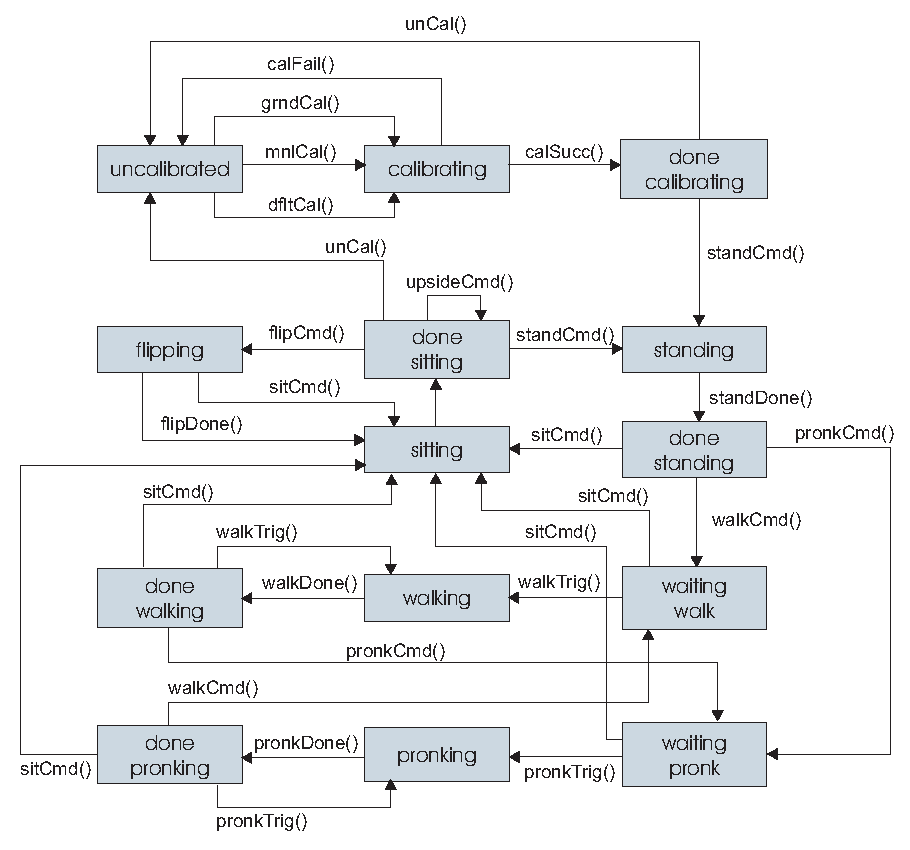
\includegraphics{SupervisorMachine.eps}}
    \caption{State transition diagram for the {\tt Supervisor} state
      machine. This machine controls the overall user interface of the {\tt
        rhex\_standard} demo program.}
    \label{fig:supervisor_machine}
  \end{center}
\end{figure}
%%%%%%%%%%%%%%%%%%%%%%%%%%%%%%%%%%%%%%%%%%%%%%%%


\subsection{The Main Executable}

